\chapter{Experimental Results And Performance Analysis}


\section{Experimental Results}
Web and mobile platform has been tested in our project. Different scenarios were applied with these tests and there was 0.02 percent error observed.

\section{Performance Analysis}

Performance tests were calculated with Apache JMeter tool which makes HTTP request simultaneously depending upon call number that we give. We monitored the CPU and RAM percentage at the server side by using HTOP tool. Different outputs for different number of calls is shown below. HTTP calls loop count is 10 and time interval between loop counts is 10 seconds.

One of the example HTTP call is shown in Figure 
\ref{fig:exampleCall}.

\begin{figure}[!htbp]
\centering
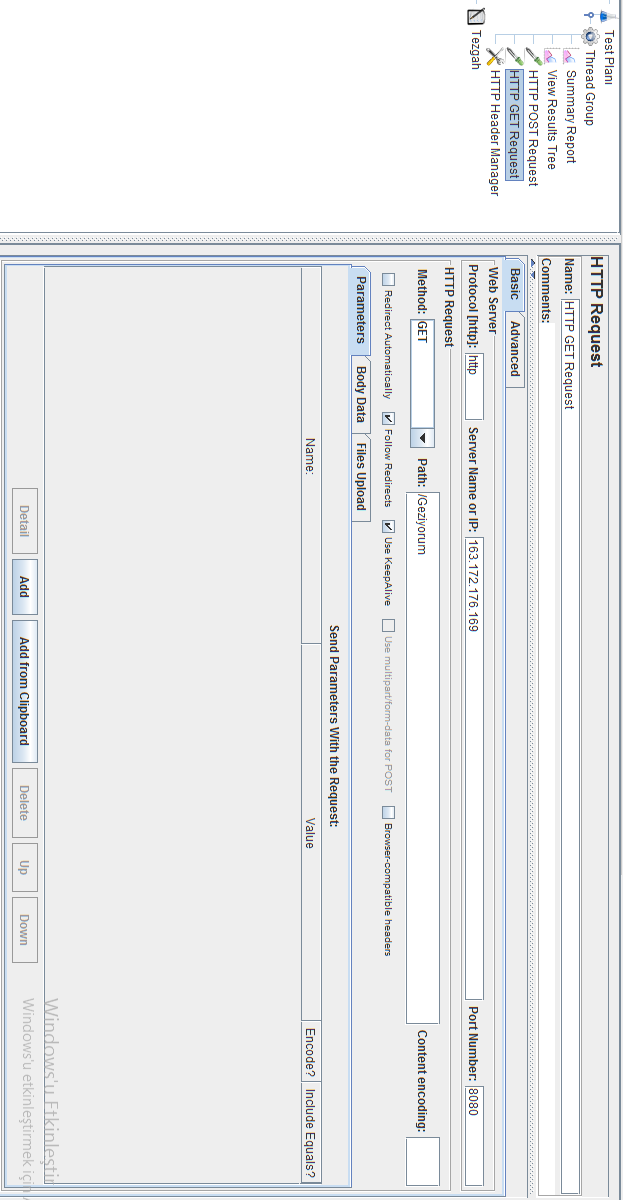
\includegraphics[width=\textwidth]{projectChapters/images/exampleCall.png}
\caption{Example HTTP call}
\label{fig:exampleCall}
\end{figure}

\newpage

Server's idle performance is shown in Figure 
\ref{fig:serveridle}.

\begin{figure}[!htbp]
\centering
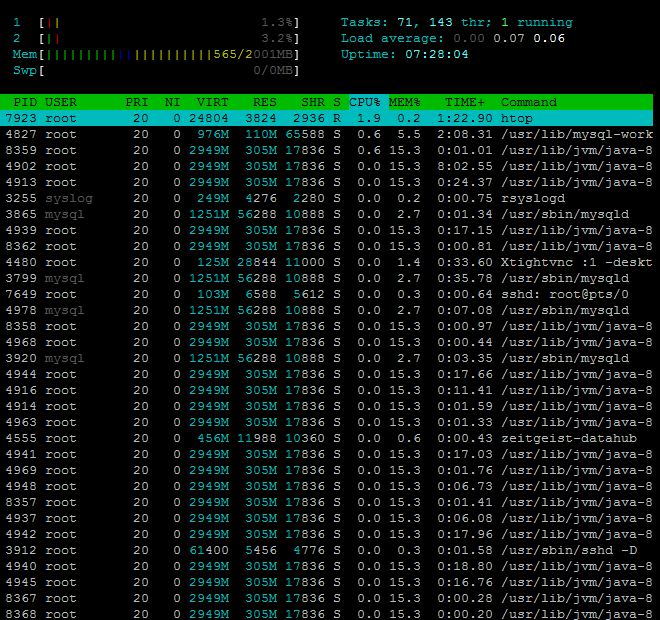
\includegraphics[width=\textwidth]{projectChapters/images/serveridle.png}
\caption{When server is idle position}
\label{fig:serveridle}
\end{figure}

\subsection{Result}




As we seen the results below, the server can handle up to 200 simultaneously HTTP calls, its bottleneck is its CPU power, because maximum RAM usage 20 percent even the highest limit of calls. If we assume that average HTTP calls per web page is 20, (the number can vary depending upon the demand of the user) as a result, if server can handle 200 simultaneous calls and user makes 20 calls per page we can say the average number of users that our server can handle is 10.

\begin{table}[!ht]
\centering
\caption{Server performance test results}
\label{my-label}
\begin{tabular}{|l|l|l|}
\hline
\textbf{HTTP Calls}                & \textbf{Maximum Memory Usage(\%)} & \textbf{Maximum CPU Usage(\%)} \\ \hline
30 GET Requests           & 15.2                     & 18.1  \\ \hline
100 GET Requests          & 15.2                     & 56.6  \\ \hline
130 GET and POST Requests & 15                       & 68.8  \\ \hline
180 GET and POST Requests & 15                       & 89.4  \\ \hline
\end{tabular}
\end{table}

\newpage

Comparison between HTTP calls and the result outputs of error rate, throughput, Received KB/sec, Sent KB/sec, Avg Bytes are shown in Figure

\ref{fig:summaryReport}.

\begin{figure}[!htbp]
\centering
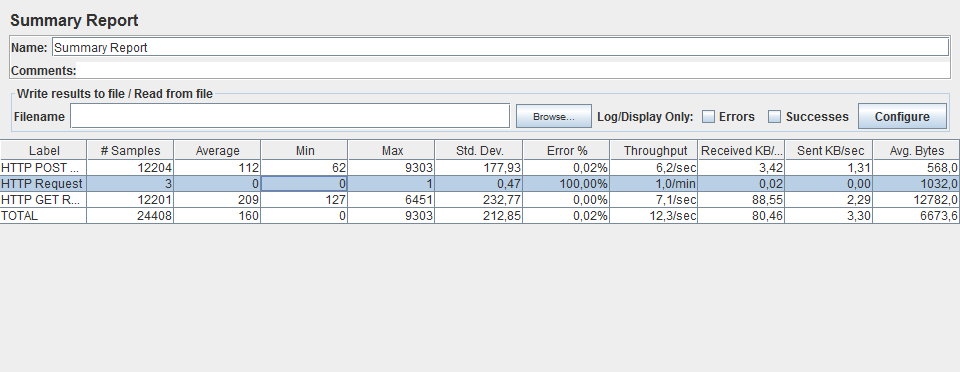
\includegraphics[width=\textwidth]{projectChapters/images/summaryReport.png}
\caption{Statistical summary report of HTTP calls}
\label{fig:summaryReport}
\end{figure}












